\section{Wavelet group disturbance and shedding}\label{sec:wavelet-group-disturbance}

\subsection*{Wave handoff}
A wave is a Markovian or retained-history entropic handoff of distinction-information through a recurring relational motif. In AOD, the local handoff form is the duon wavelet
\[
W[D_i\mu D_j],
\qquad
D_i,D_j\in\{D_\alpha,D_\Omega\},
\qquad
\mu\in\{-1,0,+1\}.
\]
A wavelet group is a carried segment of duon-current handoff. Coherent handoff preserves motif form. Lead--lag excess contributes to shedding, reclosure, or entropic duon current. \apref{app:wave}.

\begin{definition}[Wavelet group]
A wavelet group is a carried segment of duon current participating in wave handoff.
\end{definition}

\begin{definition}[Lead--lag disturbance span]
The lead--lag disturbance span is the carried asymmetric return extent of a wavelet group on the declared cut lineage.
\end{definition}

A wavelet group carries lead--lag disturbance on duon current. The carried span contributes to PADAR burden. When the span exceeds local closure compatibility, excess disturbance sheds.

\begin{definition}[PADAR burden of a wavelet group]
For a wavelet group \(W\) on a declared boundary/window, its PADAR burden is
\[
P^{\PADAR}_{W}(\partial F,\omega)=
\sum_{e\in W}
C_{3,e}
\min\!\left(D_e(\partial F,\omega),|\omega|_e\right)
\left|\Delta^{\chi\mathrm{lag}}_e\right|.
\]
Here \(|\omega|_e\) is the overlap of the declared window with the retained channel \(e\), \(D_e\) is the PADAR duration coordinate, and \(\Delta^{\chi\mathrm{lag}}_e\) is the chiral lead--lag mismatch carried by that channel.
\end{definition}

\begin{definition}[Shedding]
Shedding is the break of excess carried disturbance from local closure compatibility. If \(C^{\mathrm{close}}_W(\partial F,\omega)\) is local closure compatibility, then
\[
X_W(\partial F,\omega)=
\max\!\left(0,
P^{\PADAR}_{W}(\partial F,\omega)-C^{\mathrm{close}}_W(\partial F,\omega)
\right)
\]
records shed excess.
\end{definition}

The shed excess can move outward across a shell boundary, reclose locally, or enter a decay path. With reclosure fraction \(\lambda_{\mathrm{reclose}}\in[0,1]\), write
\[
X_W^{\mathrm{reclose}}=\lambda_{\mathrm{reclose}} X_W,
\qquad
X_W^{\mathrm{out}}=(1-\lambda_{\mathrm{reclose}})X_W.
\]
Here \(X_W^{\mathrm{out}}\) is outward shedding.

\begin{definition}[Reclosure path]
A reclosure path is a local reclosure of shed disturbance on retained support. Stable reclosure yields retained shell closure. Unstable reclosure continues as a decay path.
\end{definition}

\begin{figure}[H]
\centering
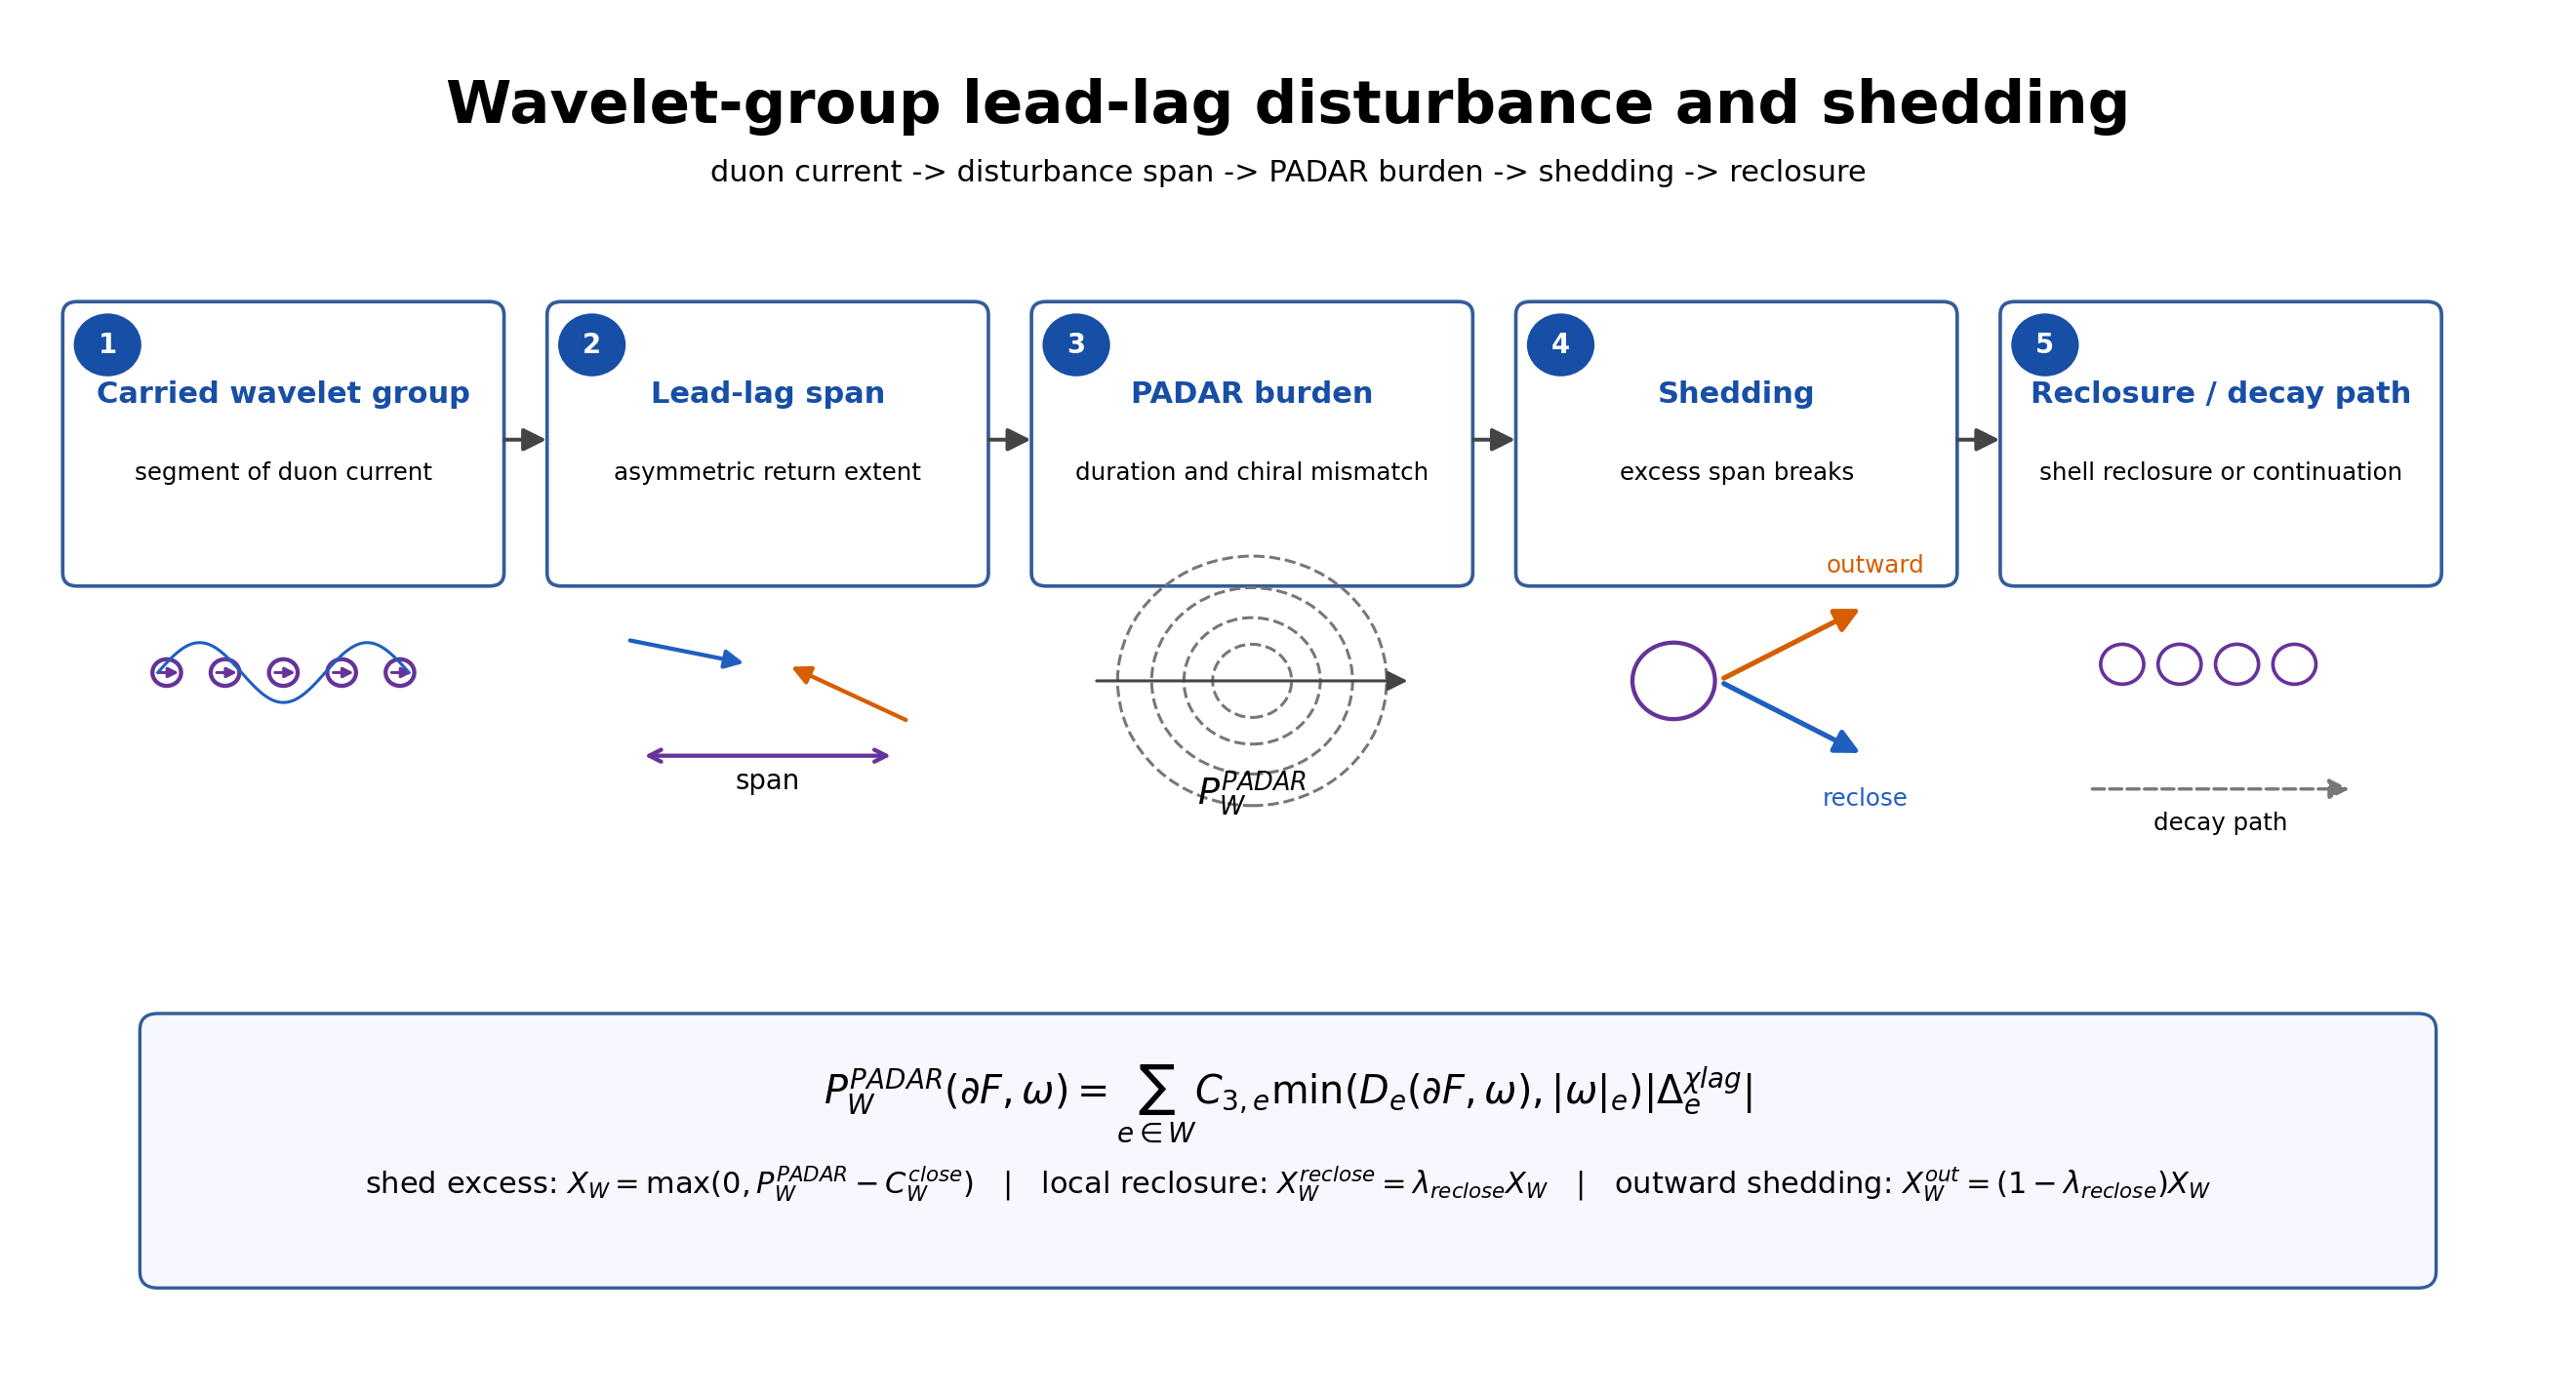
\includegraphics[width=0.98\linewidth]{figures_jpg/v39_15_wavelet_group_disturbance_shedding.png}
\caption{Wavelet-group lead--lag disturbance and shedding. A carried wavelet group transports a lead--lag disturbance span. Excess PADAR burden sheds; the split outcome is outward shedding or local shell reclosure.}
\label{fig:v39-wavelet-disturbance-shedding}
\end{figure}
